\section[Гипотезы]{Задача проверки гипотез. Виды гипотез: параметрические, 
непараметрические, простые, сложные. Основная гипотеза и 
альтернатива. Ошибки I-го и II-го рода. Оптимальный критерий 
Неймана-Пирсона}
\epigraph{\emph{Лекция 9}}

\subsection{Проверка гипотез}
Пусть $ X_1, X_2, \ldots, X_n $ --- выборка из некоторого закона распределения,
возможно зависящего от некоторых параметров.

\begin{definition}
Будем называть \emph{гипотезами} предположения относительно параметров, вида
распределения и т.\,д.
\end{definition}

\begin{definition}[характеристики гипотезы]
	Гипотеза называется \emph{параметрической}, если делаются предположения о
	значениях параметров распределения.

	Гипотеза называется \emph{непараметрической}, если делаются предположения о
	виде закона распределения, независимости признаков.

	Гипотеза называется \emph{простой}, если она однозначно определяет закон
	распределения.

	Наконец, гипотеза называется \emph{сложной}, если она неоднозначно определяет
	закон распределения.
\end{definition}

\begin{ex}
 Гипотеза $ H_0 $ --- выборка из распределения Пуассона с параметром $ \lambda = 2 $ ---
 простая параметрическая.

 Гипотеза $ H_1 $ --- выборка из нормального распределения --- сложная
 непараметрическая.

 Гипотеза $ H_2 $ --- выборка из распределения с параметром $ \theta = \theta_0
 $ --- простая параметрическая, если $ \theta \in \mathbb R $.

 Гипотеза $ H_3 $ --- выборка из нормального распределения с параметром $ a = 0
 $ --- сложная параметрическая.

 Гипотеза $ H_4 $ --- монета правильная --- простая гипотеза.

 Гипотеза $ H_5 $ --- монета неправильная --- сложная гипотеза.
\end{ex}

\subsubsection{Мотивация}
Одна из гипотез $ H_0 $ --- основная, и вместе с ней рассматривается
конкурирующая гипотеза, или \emph{альтернатива} $ H_1 $.

\begin{definition}
Пусть $ H_0 $ --- выборка из известного закона распределения с параметром $
\theta = \theta_0 $.

Альтернативу $ H_1 $: $ \theta = \theta_1 \neq \theta_0 $ назовём
\emph{простой}; альтернативу $ \theta \neq \theta_0 $ --- \emph{двусторонней};
альтернативы $ \theta < \theta_0 $ и $ \theta < \theta_0 $ назовём
\emph{односторонними}.
\end{definition}

\begin{definition}
\emph{Критерием} называется правило, по которому принимается решение, о принятии
гипотезы $H_0$, или отклонении $ H_0 $ в пользу альтернативы $ H_1 $, на основе
анализа выборки. 
\end{definition}
Критерий задаётся с помощью \emph{критического множества} $ S $ и статистики $ z
= z(X_1, X_2, \ldots, X_n)$. При этом если $ z \in S $, то гипотеза $ H_0 $
\textsl{отклоняется}, а в случае $ z \notin S$ --- \textsl{принимается}.

\begin{figure}[h!]
	\centering
	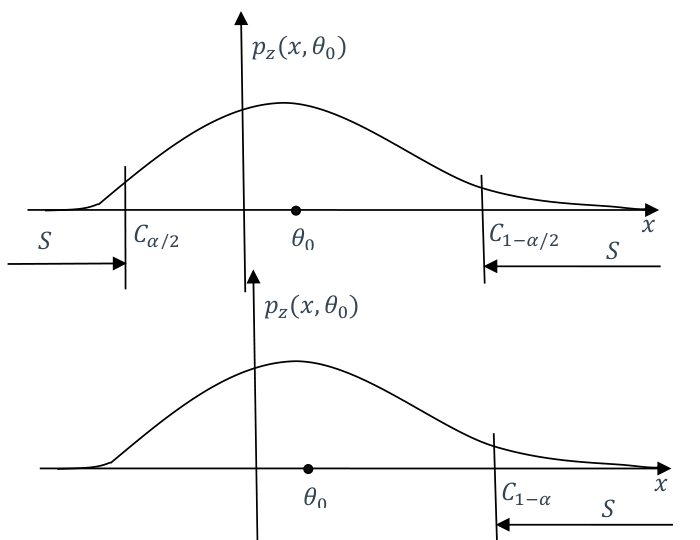
\includegraphics[width=0.8\textwidth]{Figures/9-plot1.png}
	\caption{}
	%FIXME: исправить описание
	\label{fig:9-plot1-png}
\end{figure}

\subsubsection{Ошибка первого рода}
\begin{definition}
	Условную вероятность 
	\[
			\alpha := P(z\in S \mid H_0)
	\]
назовём \emph{ошибкой первого рода}. Эта вероятность суть вероятность отклонения
верной гипотезы, \emph{уровень значимости критерия}.
\end{definition}
% отсебятина
Понятно, что чем уровень значимости критерия меньше, тем лучше сам критерий.
Понятно кроме того, что в реальных задачах критерий с нулевым уровнем
значимости существовать не может, поскольку он характеризует уже не гипотезу, а
некоторое верное утверждение и тем
самым теряет свой смысл.
 
Пусть $ H_0 $: $ \theta = \theta_0 $ --- простая гипотеза. Вид критического
множества для $ H_1 $: $ \theta \neq \theta_0 $ --- двусторонняя альтернатива.

Тогда  
\[
	S = \{z \leqslant C_{\alpha/2}\} \cup \{z \geqslant C_{1-\alpha/2}\}.
\]
В случае, когда альтернатива будет $ H_1 $: $ \theta > \theta_0 $
правосторонней, имеем  
\[
	S = \{z \geqslant C_{1-\alpha}\}.
	%FIXME: пропущено деление на два (\alpha/2)?
\]

\begin{ex}
	Пусть сопротивление резисторов $ \xi $ --- случайная величина, подчиняющаяся
	нормальному закону. Произведено $ n = 36 $
измерений, в результате чего оказалось, что $\bar X$ = 9.3\,кОм. 

Требуется проверить на уровне значимости $ \alpha = 0.05 $ гипотезу $ H_0 $: $ a = 10
$\,кОм против двусторонней альтернативы $ H_1 $: $ \theta \neq 10 $\,кОм в двух
ситуациях: а) $ \sigma^2 = 4 $\,кОм^2; b) $ S^2 = 6.25 $\,кОм^2.
\begin{solution}
	\begin{enumerate}[label=\alph*)] %TODO: буквы
	\item Как известно, статистика 
	\[
		\frac{\bar X - a}{\sigma}\cdot\sqrt{n}
	\]
	имеет стандартное нормальное распределение, то есть  
	\[
		P\left(u_{\alpha/2} \leqslant \frac{\bar X - a}{\sigma} \cdot \sqrt n \leqslant
		u_{1-\alpha/2} \right) = 1 - \alpha,
	\]
	или с учётом симметричности $ u_{\alpha/2} = -u_{1 - \alpha/2} $ нормального
	распределения  
	\[
			P \left( \left| \frac{\bar X - a}{\sigma}\cdot \sqrt n \right| \geqslant
			u_{1-\alpha/2} \right) = \alpha.
	\]

	Таким образом, поскольку $ u_{0.975} = 1.96 $, критическое множество в данном случае имеет вид
\[
		S = \left\{  \left| \frac{\bar X - a}{\sigma} \cdot \sqrt n \right| \geqslant
		u_{1-\alpha/2}\right\} = \left\{ \left| \frac{\bar X - 10}{2} \cdot 6 \right|
	\geqslant u_{0.975} \right\} = \{ \bar X \geqslant 10.65\} \cup \{\bar X
\leqslant 9.35\}.
\]
Поскольку $ \bar X = 9.3 \in S $, то гипотеза $ H_0 $: $ a = 10 $\,кОм
отклоняется на уровне значимости 0.05.
\item В этом случае используем статистику	 
\[
		\frac{\bar X - a}{S}\sqrt n,
\]
распределённую по закону Стьюдента, который также симметричен. Тогда 
\begin{align*}
	1 - \alpha &= P \left( t_{\alpha/2}(n-1)\leqslant \frac{\bar X - a}{S}\sqrt n
	\leqslant t_{1-\alpha/2}(n-1) \right),\\
	\alpha &= P \left( \left| \frac{\bar X - a}{S}\sqrt n \right| \geqslant
	t_{1-\alpha/2} (n-1) \right).
\end{align*}

Высчитав значение квантилли $ t_{0.975}(35) = 2.03 $, получим 
\[
		S = \left\{ \left| \frac{\bar X - a}{S}\sqrt n \right| \geqslant
		t_{1-\alpha/2}(n-1) \right\} = \left\{ \left| \frac{\bar X - 10}{2.5}\cdot 6
	\right| \geqslant 2.03 \right\} = \{\bar X \geqslant 10.84\} \cup \{\bar X
	\leqslant 9.15\}.
\]
В этом случае гипотеза $ H_0 $: $ a = 10 $\,кОм принимается, поскольку $ \bar X
= 9.3 \notin S$.
\end{enumerate}

\end{solution}
\end{ex}
\begin{ex}\label{ex:2}
	В условиях предыдущего примера требуется проверить на том же уровне значимости
	гипотезу $ H_0 $: $ a = 10 $\,кОм против левосторонней альтернативы $ H_1 $:
	$ a < 10 $\,кОм в двух ситуациях: a) $ \sigma^2 = 4 $\,кОм^2; b) $ S^2 = 6.25
	$\,кОм^2.
	\begin{solution}
		\begin{enumerate}[label=\alph*)]
			\item\label{enum:1} Решение этого примера  построено на той же статистике 
			\[
					\frac{\bar X - a}{\sigma}\sqrt n,
			\]
			однако критическое множество будет состоять из значений этой статистики,
			говорящих в пользу альтернативы, то есть 
			\[
				S = \left\{ \frac{\bar X - a}{\sigma}\sqrt n \leqslant - u_{1-\alpha}
				\right\} = \left\{ \frac{\bar X - a}{2} \cdot 6 \leqslant - 1.645
				\right\} = \{\bar X \leqslant 9.45 \}.
			\]
		Поскольку $ \bar X = 9.3 \in S $, то гипотеза $ H_0 $: $ a = 10 $\,кОм
		отвергается.	
	\item Аналогично предыдущему случаю, основную гипотезу нужно отвергать в случае малых 
		значений $X$. Произведем вычисления. Учитывая, что $ t_{0.95}(35) = 1.69 $,
	\[
		S = \left\{ \frac{\bar X - a}{S}\sqrt n \leqslant -t_{1-\alpha/2}(n-1)
		\right\} = \left\{ \frac{\bar X - 10}{2.5}\cdot 6 \leqslant -1.69 \right\} =
		\{\bar X \leqslant 9.296\}.
	\]
	В этом случае гипотеза $ H_0: a = 10 $\,кОм принимается, поскольку $ \bar X =
	9.3 \notin S$.
		\end{enumerate}

	\end{solution}
\end{ex}

\subsubsection{Ошибка второго рода}
\begin{definition}
Назовём условную вероятность
\[
	P(z\notin S \mid H_1) = \beta
\]
\emph{ошибкой второго рода}. Эта вероятность суть вероятность принятия неверной
гипотезы $ H_0 $ в случае простой альтернативы.
\end{definition}

\begin{definition}
Вероятность $W(S, \theta) = P_\theta(z\in S)$ называется \emph{функцией мощности
критерия}.
\end{definition}

При этом $ \alpha = W(S, \theta_0) $ --- вероятность отклонения верной гипотезы,
а $ 1-\beta = P(z \in S \mid H_1) = W(S, \theta_1) $ --- вероятность отвергнуть
неверную гипотезу.
%TODO: пояснить

%TODO: examples
\begin{ex}
	Требуется в условиях предыдущего примера проверить на том же уровне значимости
	ту же гипотезу $ H_0 $: $ a = 10 $\,кОм $ = a_0 $ против простой альтернативы
	$ H_1 $: $ a = 9 $\,кОм $ = a_1 $, если $ \sigma^2 = 4 $\,кОм^2. 
	\begin{solution}
		Поскольку $ a_1 < a_0 $, критическое множество совпадает с найденным в
		примере \ref{ex:2} п. \ref{enum:1}:  
		\begin{equation}\label{eq:1}
			S = \{\bar X \leqslant 9.45\},
		\end{equation}
		что даёт основания отвергнуть $ H_0 $ и принять $ H_1 $. 

		Вычислим ошибку	второго рода: 
		\begin{multline*}
				\beta = P(z \notin S \mid H_1) = P(\bar X > 9.45 \mid a = 9) =\\= P \left(
				\frac{\bar X - a}{\sigma}\sqrt n > \frac{9.45 - a}{\sigma}\sqrt n \mid a
			= 9\right) = P \left( \frac{\bar X - 9}{2} \cdot 6 > 1.35 \right) = 1 -
			\Phi(1.35) = 0.0885.
		\end{multline*}

	\end{solution}
\end{ex}
\begin{ex}
	В условиях предыдущего примера для того же уровня значимости требуется найти
	ошибку второго рода при проверке гипотезы $ H_0 $: $ a =10 $\,кОм $ = a_0 $
	против простой альтернативы $ H_1 $: $ a = 9.5 $\,кОм $ = a_1 $, если $
	\sigma^2 4 $\,кОм^2.
	\begin{solution}
		Поскольку $ a_1 < a_0 $, критическое множество будет тем же \eqref{eq:1},
		что даёт основания отвергнуть $ H_0 $ и принять $ H_1 $.

		Вычислим ошибку второго рода: 
		\[
				\beta = P(z\notin S\mid H_1) = P(\bar X > 9.45 \mid a = 9.5) = P \left(
				\frac{\bar X - a}{\sigma}\sqrt n> \frac{9.45 - a}{\sigma} \sqrt n\mid a
			= 9.5\right) = P \left( \frac{\bar X - 9}{2}\cdot 6 > -0.15 \right) =
			\Phi(0.15) = 0.56.
		\]

	\end{solution}	
\end{ex}
\begin{ex}
	В условиях предыдущих примеров для того же уровня значимости требуется найти
	функцию мощности левостороннего критерия при проверке гипотезы $ H_0 $: $ a =
	10$\,кОм $ = a_0 $ против простой альтернативы $ H_1 $: $ a = a_1 < a $, если
	$ \sigma^2 = 4 $\,кОм^2.
\begin{solution}
	По определению мощность критерия \eqref{eq:1} против альтернативы $ H_1 $: $ a
	= a_1 < 10$ можно вычислить следующим образом: 
	\[
			W(S, a_1) = P(\bar X \leqslant 9.45\mid H_1) = P \left( \frac{\bar X -
			a_1}{\sigma} \sqrt n \leqslant \frac{9.45 - a_1}{\sigma} \sqrt n \right) =
			\Phi = \left( \frac{9.45 - a_1}{\sigma}\sqrt n \right).
	\]
	\begin{figure}[h!]
		\centering
		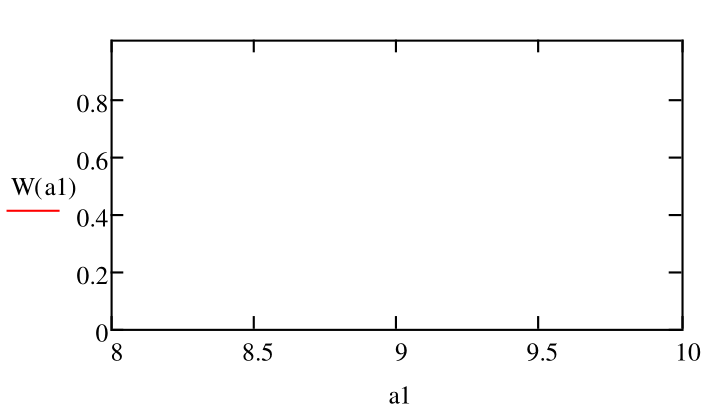
\includegraphics[width=0.8\textwidth]{Figures/9-plot2.png}
		\caption{}
		\label{fig:9-plot2}
	\end{figure}
	%FIXME: странный рисунок

\end{solution}
\end{ex}

\textsc{Вывод}.
Для построенного критерия в случае простой альтернативы ошибка второго рода 
вычисляется однозначно. 
 Большая ошибка второго рода говорит о низкой мощности критерия, он плохо различает 
близкие гипотезы. 

\subsubsection{Возможные задачи}
\begin{enumerate}
	\item Для данной альтернативы найти максимально мощный (оптимальный) критерий
		$ S^\ast $, то есть  
		\[
				W(S^\ast, \theta) = \max_S W(S,\theta).
		\]
	\item Для построенного критерия выбрать такую альтернативу, чтобы достигнуть
		максимальной мощности.
	\item Найти необходимый объём выборки, обеспечивающий заданную мощность
		критерия при заданных основной и альтернативной гипотезах.
\end{enumerate}


\subsection{Улучшение критерия за счёт увеличения объёма наблюдений}
Положим требуется найти минимальный объём выборки, удовлетворяющей условиям 
\begin{align*}
	H_0: a &= 10\text{\,кОм} = a_0,\\
	H_1: a &= 9.5\text{\,кОм} = a_1 < a_0,\\
	\sigma^2 &= 4\text{кОм}^2,\\
	\alpha &= 0.05, \quad \beta\leqslant0.1.
\end{align*}
\begin{solution}
	В рассматриваемой ситуации критическое множество имеет вид $ S = \{\bar X
	\leqslant C\} $. По условию 
	\begin{align*}
		0.05 &= P(z\in S\mid H_0) = P(\bar X \leqslant C \mid a = 10) = \Phi \left(
			\frac{C - 10}{2} \sqrt n\right),
			0.1 &\geqslant P(z \in \bar S \mid H_1) = P(\bar X > C \mid a = 9.5) = 1 -
		\Phi \left( \frac{C - 9.5}{2}\sqrt n \right).
	\end{align*}
Решая эту систему, находим $ n \geqslant 138 $.
\end{solution}

\textsc{Вывод}.  При увеличении числа наблюдений хорошая оценка (например та, для которой 
выполнены достаточные условия состоятельности $\D \widehat \theta_n \to 0$) по
вероятности (а значит, и 
по распределению) сходится к истинному значению параметра, то есть к неслучайной 
величине, что позволяет различить даже близкие простые гипотезы. 


\subsection{Оптимальный критерий Неймана -- Пирсона}
	С каждым критерием $ S $ свяжем функцию  
	\[
		\varphi(\vec X_n) = \begin{cases} 1, &z(\vec X_n) \in S,\\
		0, &z(\vec X_n) \notin S.\end{cases}
	\]
Тогда  
\begin{gather*}
	W(S, \theta) = W(\varphi(\vec X_n), \theta) = P_\theta(z(\vec X_n) \in S) =
	M_\theta(\varphi(\vec X_n)) = \int \varphi(\mathbf x) p(\mathbf x,
	\theta)\,d\mathbf x,\\
	W(S,\theta_0) = \alpha, \qquad W(S,\theta_1) = 1 - \beta.
\end{gather*}

\begin{theorem}[критерий отношения правдоподобия]\label{th:N-P}
	Рассмотрим множество критериев уровня $ \alpha $ для проверки гипотезы $ H_0
	$: $ \theta = \theta_0 $ против простой альтернативы $ H_1 $: $ \theta =
	\theta_1 $, $ \theta_1 \neq \theta_0 $. Тогда для любого $ 0 < \alpha < 1 $
	существуют такие числа $ c \geqslant 0 $ и $ \varepsilon \in [0, 1] $, что
	критерий с функцией  
	\[
	\varphi^\ast(\vec X_n) = \begin{cases} 1, & \frac{\mathscr L(\vec X_n,
		\theta_1)}{\mathscr L(\vec X_n, \theta_0)} > c,\\[0.4em]
		\varepsilon, & \frac{\mathscr L(\vec X_n, \theta_1)}{\mathscr L(\vec X_n, \theta_0)} =
		c,\\[0.4em]
		0, & \frac{\mathscr L(\vec X_n, \theta_1)}{\mathscr L(\vec X_n, \theta_0)} < c
	\end{cases}
	\]
является оптимальным (наиболее мощным) во множестве критериев уровня $ \alpha $.	
\end{theorem}
\begin{proof}
%TODO: proof
\end{proof}

\begin{ex} 
	Пусть выборка объёма $ n = 100 $ подчинена показательному закону с параметром
	$ \lambda $. Установим вид оптимального критического множества для проверки
	гипотезы $ H_0 $: $ \lambda = \lambda_0 $ против простой альтернативы $ H_1 $:
	$ \lambda = \lambda_1 $, если $ \lambda_1 > \lambda_0 $.
  \begin{solution}
		Согласно теореме \ref{th:N-P} оптимальное критическое множество имеет вид 
		\[
				\frac{\mathscr L(\vec X_n, \lambda_1)}{\mathscr L(\vec X_n, \lambda_0)} > c,
		\]
		откуда  
		\[
				\frac{\mathscr L(\vec X_n, \lambda_1)}{\mathscr L(\vec X_n, \lambda_0)} =
				\frac{\prod^n_{k=1} \lambda_1 e^{-\lambda_1 X_k}}{\prod_{k=1}^n
				\lambda_0 e^{-\lambda_0 X_k}} = \left( \frac{\lambda_1}{\lambda_0}
			\right)^n \exp\left[-\left(\lambda_1 - \lambda_0\right) \sum_{k=1}^n X_k\right] \geqslant c.
		\]
		Разрешим это неравенство относительно $ \sum_{k=1}^n X_k $ (достаточная
		статистика!): 
		\begin{align*}
				\exp\left[-\left(\lambda_1 - \lambda_0\right) \sum_{k=1}^n X_k\right]
				&\geqslant c \left( \frac{\lambda_0}{\lambda_1} \right)^n,\\
        -(\lambda_1 - \lambda_0) \sum_{k=1}^n X_k &\geqslant \ln \left[ c \left(
				\frac{\lambda_0}{\lambda_1}\right)^n  \right],\\
						\sum_{k=1}^n X_k &\leqslant \frac{\ln c + n \ln
				(\lambda_0/\lambda_1)}{\lambda_0 - \lambda_1} = c_1.
		\end{align*}

	\end{solution}	
\end{ex}

\begin{ex}
	\begin{enumerate}
		\item Построим критерий на уровне $ 1 - \alpha = 0.95 $ для различения
			гипотез о параметре показательного закона на основе выборки объёма $ n =
			100 $, где 
			\begin{align*}
				H_0: \lambda &= \frac{1}{3},\\
				H_1: \lambda &= \frac{5}{11}.
			\end{align*}
			\begin{solution}
				Согласно критерию Неймана -- Пирсона $ S = (\bar X \leqslant C) $.
				Далее, 
				\[
						\alpha = P(\bar X \in S \mid H_0 ) = P(\bar X \leqslant C \mid H_0)
						= P \left( 2\lambda_0 \sum_{k=1}^n X_k \leqslant 2\lambda_0 n C
						\right) = F_{\chi^2(2n)}(2\lambda_0 n C).
				\]
				Значит, $ 2\lambda_0 n C = \chi^2_\alpha(2n) $, а значит, 
				\[
						C = \frac{\chi^2_\alpha(2n)}{2\lambda_0 n} = 2.524.
				\]

			\end{solution}
			
			\item Найдём ошибку второго рода построенного критерия.
				\begin{solution}
				\[
					\beta = P(\bar X > C \mid H_1 ) = P \left( 2\lambda_1 \sum_{k=1}^n X_k
					> 2\lambda_1 n C\right) = 1 - F_{\chi^2(2n)}(2\lambda_0 n C) = 0.075.
				\]

			\end{solution}

		\item Найдём объём выборки, обеспечивающий при решении задачи о различении
			этих гипотез ошибки $ \alpha = 0.05 $ и $ \beta = 0.05 $.

			\begin{solution}
			Согласно критерию Неймана -- Пирсона $ S = (\bar X \leqslant C) $. Тогда
			при больших $ n $ имеем  
			\begin{align*}
				\alpha &= P(\bar X \in S\mid H_0) = P(\bar X \leqslant C \mid H_0) = P
					\left( \frac{n\bar X - 1/\lambda_0}{\sqrt{n/\lambda^2_0}}\leqslant
					\frac{nC - n/\lambda_0}{\sqrt{n/\lambda^2_0}} \right) \approx \Phi
					\left( \frac{n C \lambda_0 - n}{\sqrt n} \right),\\ 
				\beta &= P(\bar X \notin S \mid H_1) = P(\bar X > C \mid H_1) = P
					\left( \frac{n\bar X - 1/\lambda_1}{\sqrt{n/\lambda^2_1}}\leqslant
					\frac{nC - n/\lambda_1}{\sqrt{n/\lambda^2_1}} \right) \approx \Phi
					\left( \frac{n C \lambda_1 - n}{\sqrt n} \right).
			\end{align*}
			
			Решим полученную систему: 
			\[
				\begin{cases}
					C \lambda_0 \sqrt n - \sqrt n = u_\alpha,\\
					C\lambda_1 \sqrt n - \sqrt n = u_{1-\beta}.
				\end{cases}
				\implies
				\begin{cases}
					\sqrt n = \frac{u{1-\beta}\lambda_0 - u_\alpha \lambda_1}{\lambda_1 -
					\lambda_0},\\
					C = \frac{\sqrt n + u_\alpha}{\lambda_0\sqrt n}.
				\end{cases}
				\implies
				\begin{cases}
					n \approx 115, \\
					C = 2.538.
				\end{cases}
			\]

		\end{solution}
	\end{enumerate}
\end{ex}
	
